%%
%% Copyright 2007, 2008, 2009 Elsevier Ltd
%%
%% This file is part of the 'Elsarticle Bundle'.
%% ---------------------------------------------
%%
%% It may be distributed under the conditions of the LaTeX Project Public
%% License, either version 1.2 of this license or (at your option) any
%% later version.  The latest version of this license is in
%%    http://www.latex-project.org/lppl.txt
%% and version 1.2 or later is part of all distributions of LaTeX
%% version 1999/12/01 or later.
%%
%% The list of all files belonging to the 'Elsarticle Bundle' is
%% given in the file `manifest.txt'.
%%

%% Template article for Elsevier's document class `elsarticle'
%% with numbered style bibliographic references
%% SP 2008/03/01
%%
%%
%%
%% $Id: elsarticle-template-num.tex 4 2009-10-24 08:22:58Z rishi $
%%
%%
\documentclass[preprint,10pt,5p]{elsarticle}

\usepackage[portuguese]{babel}

%% Use the option review to obtain double line spacing
%\documentclass[preprint,review,12pt]{elsarticle}

%% Use the options 1p,twocolumn; 3p; 3p,twocolumn; 5p; or 5p,twocolumn
%% for a journal layout:
%% \documentclass[final,1p,times]{elsarticle}
%% \documentclass[final,1p,times,twocolumn]{elsarticle}
%% \documentclass[final,3p,times]{elsarticle}
%% \documentclass[final,3p,times,twocolumn]{elsarticle}
%% \documentclass[final,5p,times]{elsarticle}
%% \documentclass[final,5p,times,twocolumn]{elsarticle}

%% if you use PostScript figures in your article
%% use the graphics package for simple commands
%% \usepackage{graphics}
%% or use the graphicx package for more complicated commands
%% \usepackage{graphicx}
%% or use the epsfig package if you prefer to use the old commands
%% \usepackage{epsfig}

%% The amssymb package provides various useful mathematical symbols
\usepackage{amssymb}
%% The amsthm package provides extended theorem environments
%% \usepackage{amsthm}

%% The lineno packages adds line numbers. Start line numbering with
%% \begin{linenumbers}, end it with \end{linenumbers}. Or switch it on
%% for the whole article with \linenumbers after \end{frontmatter}.
\usepackage{lineno}
\usepackage{amsmath}

\usepackage{amsmath}
\usepackage{algorithm}
\usepackage[noend]{algpseudocode}

%% Acrescentei o pacote abaixo para usar subfigures mas talvez não seja recomendado...
\usepackage{subcaption}

%% Acrescentei este pacote aqui para linhas duplas em tabelas sem cortes
\usepackage{hhline}

%% Acrescentei este pacote para permitir links clicáveis
\usepackage{hyperref}

\usepackage{microtype}

%% natbib.sty is loaded by default. However, natbib options can be
%% provided with \biboptions{...} command. Following options are
%% valid:

%%   round  -  round parentheses are used (default)
%%   square -  square brackets are used   [option]
%%   curly  -  curly braces are used      {option}
%%   angle  -  angle brackets are used    <option>
%%   semicolon  -  multiple citations separated by semi-colon
%%   colon  - same as semicolon, an earlier confusion
%%   comma  -  separated by comma
%%   numbers-  selects numerical citations
%%   super  -  numerical citations as superscripts
%%   sort   -  sorts multiple citations according to order in ref. list
%%   sort&compress   -  like sort, but also compresses numerical citations
%%   compress - compresses without sorting
%%
%% \biboptions{comma,round}

% \biboptions{}

\usepackage{booktabs}

\begin{document}

\begin{frontmatter}

\title{Implementação Computacional de um Modelo para Otimização da Movimentação de Contêineres em Linhas de Cabotagem}

\address[label1]{Escola Politécnica da Universidade de São Paulo, São Paulo, Brazil}

\author[label1]{Enzo Klautau Gomes}
\ead{e\_k\_g@usp.br}

\author[label1]{Lucas Cremaschi}
\ead{lucas.cremaschi@usp.br}

\begin{abstract}
A cabotagem desempenha um papel fundamental na logística brasileira, conectando portos ao longo do extenso litoral do país e promovendo alternativas mais sustentáveis e econômicas ao transporte rodoviário. Este trabalho apresenta a implementação de um modelo computacional para otimização do transporte de contêineres nesse modal, utilizando programação em Python e o solver Gurobi. O modelo busca maximizar a margem de contribuição bruta dos fretes, considerando fatores como custos operacionais, demanda por transporte, capacidade dos navios e restrições portuárias. Além disso, foram realizadas análises de sensibilidade para avaliar o impacto de variáveis, como preço de combustíveis e taxa de câmbio, no desempenho econômico do serviço. Os resultados obtidos demonstram a aplicabilidade do modelo na tomada de decisão estratégica, contribuindo para a eficiência do transporte marítimo e a redução de custos na cadeia logística.
\end{abstract}

% The first keyword should be selected from the list of EJOR Keywords.
% Please include up to 4 additional keywords of your choice.

\begin{keyword}
Cabotagem \sep Otimização \sep Transporte de contêineres \sep Programação matemática \sep Análise de sensibilidade \sep Logística marítima \sep Modelagem matemática \sep Análise econômica \sep Transporte marítimo sustentável \sep Logística integrada \sep Otimização de rotas
\end{keyword}



\end{frontmatter}

\section{Introdução}
\label{sec:intro}

A cabotagem, modalidade de transporte marítimo ao longo da costa, exerce um papel crucial na logística brasileira, conectando portos e promovendo uma alternativa sustentável e econômica ao modal rodoviário predominante. O Brasil, com um litoral de aproximadamente 7.500 km, possui um enorme potencial para o desenvolvimento desse modal, que se destaca por apresentar menores emissões de CO2, maior eficiência energética e capacidade de movimentar grandes volumes de carga. No entanto, desafios como a predominância do transporte rodoviário, infraestrutura portuária limitada e dependência de embarcações estrangeiras ainda restringem seu pleno desenvolvimento.

A Lei da Cabotagem (Lei 9.432/1997) e iniciativas como o programa \textit{BR do Mar} têm buscado impulsionar o setor, permitindo maior flexibilidade no uso de embarcações estrangeiras, reduzindo custos operacionais e simplificando procedimentos burocráticos. Apesar disso, há necessidade de planejamento mais eficiente para superar barreiras e maximizar os benefícios do modal.

Neste contexto, este trabalho visa a implementação de um modelo computacional para otimização do transporte de contêineres em linhas de cabotagem, utilizando programação em Python e o solver Gurobi. O modelo proposto integra parâmetros como demanda, custos operacionais, capacidades de transporte e restrições logísticas, buscando maximizar a margem de contribuição bruta dos fretes e avaliar o impacto de variáveis econômicas e operacionais.

A pesquisa também inclui análises de sensibilidade, variando parâmetros como custos intermodais, preços de combustíveis e taxas de câmbio. Os resultados esperados visam não apenas otimizar o desempenho operacional e econômico, mas também contribuir para o fortalecimento da cabotagem como solução estratégica para a logística brasileira.

Diferente de Zheng et al. (2014)\cite{zhen2014} e Gençer \& Demir (2020)\cite{gencer2020}, que focam ECR isolado, este trabalho maximiza margem considerando frota realista e análise 5 anos sob BR do Mar.


\section{Revisão da Literatura}
\label{sec:literatura}

A otimização de rotas e reposicionamento de contêineres em cabotagem tem sido amplamente estudada, com ênfase em modelos matemáticos e impactos regulatórios \cite{zhen2014,gencer2020}.

\subsection{Modelos de Otimização de Rotas e Reposicionamento}

Zheng et al. \cite{zhen2014} analisam o impacto de legislações de cabotagem em redes liner shipping via programação matemática em duas fases para design hub-and-spoke (65 citações, EJOR). Conclusão: restrições regulatórias elevam custos em 15-25\%; otimização reduz empty repositioning em 12\%.

Gençer \& Demir \cite{gencer2020} desenvolvem MILP determinístico e programação estocástica para minimizar custos de empty container repositioning (ECR), considerando múltiplos tipos de contêineres e incerteza de demanda (dados reais de carrier turco, 44 semanas). MILP economiza 8,76\% vs práticas reais; SP robusto atinge 2,99\% sob incerteza.

Furlanetto et al. \cite{furlanetto2020} otimizam redes logísticas com alocação de facilities no Brasil, integrando modais. Redução de 18\% nos custos logísticos; tributos como 22\% dos gargalos (6 citações).

\subsection{Desempenho Portuário e Competitividade}

Análise DEA \cite{portos2018} revela portos brasileiros 30-40\% menos eficientes que benchmarks globais devido a burocracia e infraestrutura. Journal of Transport Geography \cite{jtg2025} demonstra cabotagem competitiva $>$800km via supernetwork multimodal, mas limitada a 12\% market share.

\subsection{Lacunas e Contribuição do Presente Trabalho}

Modelos determinísticos \cite{zhen2014} superam estocásticos \cite{gencer2020} em velocidade, mas falham em incerteza; foco regulatório vs operacional. Diferente desses trabalhos, propomos maximização de margem de contribuição com frota homogênea (4 navios semanais), sensibilidade econômica (dólar/combustível) e dados cabotagem Brasil 2025, expandindo Gençer (2020) para planejamento estratégico plurianual \cite{gencer2020,zhen2014}.


\section{Especificação do problema}

O foco principal do estudo é a implementação do modelo de otimização de rotas em Python e análise financeira dada uma rota de transporte de contêineres via modal cabotagem, com o objetivo de maximizar a margem de contribuição bruta dos fretes, considerando a variação de alguns parâmetros estabelecidos. O modelo considerado  \cite{costa2006modelo} aborda as variáveis necessárias para o desenvolvimento do caso especificado. Os principais componentes do problema estão descritos a seguir:

A demanda por transporte contêineres, os tempos de viagem, a capacidade de carga do navio, os custos fixos e variáveis estão entre os elementos que compõem a dinâmica do problema estudado. Estes fornecem a base sobre a qual a função objetivo é construída. Por exemplo, para maximizar a margem de contribuição, levará em consideração as receitas (medidas pelos parâmetros de frete para vários tipos de carga e rotas) e os custos (medidos pelos custos de operação, como tarifas portuárias e combustível).

As restrições impostas pelo modelo garantem que as soluções obtidas sejam viáveis e respeitem as limitações físicas e operacionais do sistema. Restrições de capacidade do navio, restrições de estoque de contêineres vazios, restrições de demanda, restrições de tempo e sincronização entre diferentes etapas de transporte, além de exigências legais ou contratuais, são algumas dessas limitações. Essas restrições são formuladas matematicamente e integradas ao modelo para garantir que qualquer solução sugerida pela função objetivo seja realista. Uma restrição, por exemplo, pode garantir que a quantidade de contêineres transportados em uma rota específica não exceda a capacidade de carga do navio designado para essa rota.

A função objetivo usa os valores dos parâmetros para encontrar a melhor solução possível dentro dos limites impostos pelas restrições.

A descrição do problema abordará as seguintes fatores:

\begin{itemize}
\item Rota do Navio(Southbound e Northbound): Manaus, Pecém, Suape, Santos e Paranaguá
\end{itemize}

\begin{figure} [H]
    \centering
    \caption{Portos da rota definida}
    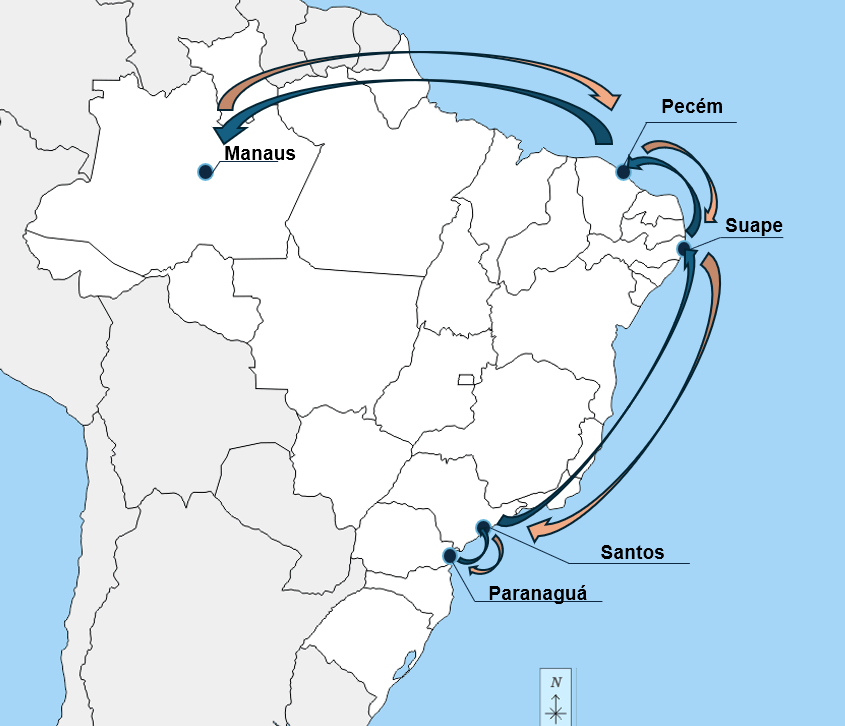
\includegraphics[width=1\linewidth]{figures/mapa cabotagem.png}
    \caption*{Fonte: Autoria própria}
    \label{fig:pot_SMCR}
\end{figure}

\begin{itemize}

     \item Portos de Escala e Tempos de Trânsito: Cada porto da rota tem suas próprias despesas operacionais, incluindo taxas portuárias, custos de manuseio de cargas e taxas de atracação, além da produtividade na movimentação de contêineres que impacta o tempo operacional do porto. Ainda, as distâncias entre os portos são fatores importantes para o planejamento de rotas, já que têm um efeito sobre os custos de combustível.
    \item Custos de Embarque e Desembarque: Os preços de embarque e desembarque de contêineres cheios ou vazios variam de um porto para outro.
    \item Calados Máximos: Existem restrições físicas que limitam o tamanho dos navios que podem atracar em cada porto. Isso afeta a escolha de um navio e a quantidade de carga que pode ser transportada.
    \item Tempo Total da Rota: O tempo total da rota (operações portuárias e viagem) é importante para garantir que o navio cumpra seu cronograma (janelas de atracação) e atenda a demanda no prazo. Ressalta-se que o serviço proposto terá um ciclo mensal.
    \item Capacidade dos Navios: Representa a capacidade dos navios em termos de deadweight (peso morto) e TEU (espaço ocupado a vinte pés). O peso morto refere-se ao peso total que um navio pode transportar, incluindo carga, combustível, água, tripulação e outros itens. Será considerado nesse estudo uma frota homogênea, composta por navios com características comuns. Isso torna o modelo mais simples e facilita a análise.
    \item Quantidade Máxima de Contêineres de 40 Pés: O número máximo de contêineres de 40 pés que podem ser alocados no navio é importante porque trata-se dotipo de contêineres mais comuns quando  há transporte de cargas volumosas.
    \item Tomadas para Contêineres Frigoríficos: Para transportar cargas perecíveis ou sensíveis à temperatura, é necessário ter tomadas para contêineres frigoríficos disponíveis.
\end{itemize}

Demanda por Carga:

\begin{itemize}

    \item Demanda por Tipo de Carga: A demanda por diferentes tipos de carga, como commodities, produtos manufaturados e produtos químicos, deve ser atendida para otimizar a capacidade do navio.
    \item Tipo de Contêiner: Diferentes tipos de carga exigem diferentes tipos de contêiner. Contêineres padrão, refrigerados e de alta capacidade são exemplos de tipos de contêineres.
    \item Tarifas de Frete: A receita que o transporte gera é influenciada pelas tarifas de frete por tipo de carga e contêiner. Tarifas mais altas entre determinados portos podem justificar o porquê de serem priorizadas na alocação de espaço.
    \item Custos de Atendimento: Os custos de atendimento por tipo de carga incluem despesas operacionais específicas, como seguro, conformidade regulamentar e manuseio especial.
    \item Pesos por Tipo de Carga e Contêiner: O peso das cargas deve respeitar o deadweight do navio.
\end{itemize}


Administração de Contêineres Vazios:

\begin{itemize}

    \item Movimentação de Contêineres Vazios: Os contêineres vazios devem ser reposicionado para manter a operação, pois há portos que exportam mais carga do que importam, reduzindo a quantidade de contêineres em estoque. Esse reposicionamento deve ser otimizado de forma a reduzir os custo associados e respeitar a capacidade do navio em serviço.

    \item Armazenagem em Portos: Contêineres vazios armazenados aumentam os custos operacionais do serviço. Por isso, é desejável manter apenas o necessário para garantir a continuidade da operação.

\end{itemize}

\section{Modelagem matemática}


\subsection{Formulação Matemática do Problema}
Para resolver o problema de otimização, propõe-se a formulação de um modelo matemático que maximiza a margem de contribuição bruta, baseando-se no no capítulo 5 da publicação de mestrado "MODELO DE MARGEM DE CONTRIBUIÇÃO APLICADO AO PLANEJAMENTO DE MARKETING NO 
TRANSPORTE MARÍTIMO REGULAR DE CONTÊINERES." \cite{costa2006modelo}. 

A função objetivo, descrição de índices, parâmetros e as restrições do modelo são apresentadas a seguir:


\subsubsection{Nomenclatura dos índices:}

\begin{itemize}
    \item \textit{i} - índice para representar os portos em uma condição de embarque dos contêineres;
    \item \textit{j} - índice para representar os portos em uma condição de desembarque dos contêineres;
    \item \textit{k} - índice para representar os tipos de contêiner;
    \item \textit{c} - índice para classificação dos tipos de carga;
    \item \textit{t} - índice para indicar o período de tempo;
    \item \textit{$\delta$} - índice para indicar os períodos de tempo antecessores aos de índice \textit{t};
    \item \textit{P} - conjunto de todos os portos;
    \item \textit{I} - conjunto de todos os portos em que há embarque de contêiner;
    \item \textit{J} - conjunto de todos os portos em que há desembarque de contêiner;
    \item \textit{K} - conjunto de todos os tipos de contêiner;
    \item \textit{$K^R$} - subconjunto de \textit{K} ($K^R \subset K$) com todos os contêineres do tipo refrigerado;
    \item \textit{$K^F$} - subconjunto de \textit{K} ($K^F \subset K$) com todos os contêineres do tamanho de 40 pés;
    \item \textit{C} - conjunto de todos os tipos de carga;
    \item \textit{T} - conjunto de todos os períodos de tempo;
    \item \textit{$\Delta$} - conjunto com todos os períodos de tempo antecessores do índice \textit{t}.
\end{itemize}
\subsubsection{Nomenclatura dos parâmetros}



\begin{itemize}
    \item \(D_{i,j,k,c,t}^{F}\) – demanda de contêineres do tipo de índice \(k\), com carga do tipo de índice \(c\), do porto de embarque de índice \(i\) para o porto de desembarque de índice \(j\), no período de tempo de índice \(t\);
    \item \(R_{i,j,k,c,t}^{F}\) – receita (frete+taxas), para uma unidade de contêiner do tipo de índice \(k\), carregando uma carga do tipo de índice \(c\), do porto de embarque de índice \(i\) para o porto de desembarque de índice \(j\), no período de tempo de índice \(t\);
    \item \(C_{i,j,k}^{F}\) – custo de embarque e desembarque de um contêiner cheio do tipo de índice \(k\), indo do porto de embarque de índice \(i\) para o porto de desembarque de índice \(j\);
    \item \(C_{i,j,k}^{E}\) – custo de embarque e desembarque de um contêiner vazio do tipo de índice \(k\), indo do porto de embarque de índice \(i\) para o porto de desembarque de índice \(j\);
    \item \(C_{c}^{M}\) – custo de atendimento ao tipo de carga de índice \(c\);
    \item \(C_{k}^{S}\) – custo de manter em estoque um contêiner do tipo de índice \(k\), por um período de tempo equivalente a um mês;
    \item \(W_{k,c}^{F}\) – peso médio dos contêineres cheios do tipo de índice \(k\) e com carga do tipo de índice \(c\);
    \item \(W_{k}^{E}\) – peso médio dos contêineres vazios do tipo de índice \(k\);
    \item \(H_{p}\) – deadweight de carga máximo no porto de índice \(p\);
    \item \(M_{p,i,j}\) – matriz de precedência. Esta matriz indica, com valores binários, quais os contêineres, com origem nos portos de embarque de índice \(i\) e com destino aos portos de desembarque de índice \(j\), estão no navio na entrada no porto de índice \(p\). Isto é, \(M_{p,i,j} = 1\), se um contêiner embarcado no porto de índice \(i\) com destino ao porto de índice \(j\) está no navio quando este chega ao porto \(p\), e zero em caso contrário;
    \item \(S_{j,i,k,\delta}^{F}\) – representa a fração de contêineres do tipo de índice \(k\) que, embarcados cheios no porto de índice \(i\) e desembarcados no porto de índice \(j\), retornam vazios a este porto depois de \(\delta\) períodos de tempo, contados a partir do embarque no porto de índice \(i\);
    \item \(S_{j,i,k,\delta}^{E}\) – representa a fração de contêineres do tipo de índice \(k\) que, embarcados vazios no porto de índice \(i\) e desembarcados no porto de índice \(j\), ficam disponíveis para utilização depois de \(\delta\) períodos de tempo, contados a partir do embarque no porto de índice \(i\);
    \item \(L_{j,k,\delta}^{F}\) – representa a fração de contêineres do tipo de índice \(k\) que, liberados para exportação a partir do terminal de contêineres vazios no porto de índice \(j\), retornam cheios a este porto depois de \(\delta\) períodos de tempo, contados a partir da liberação;
    \item \(L_{j,k,\delta}^{E}\) – representa a fração de contêineres do tipo de índice \(k\) que, liberados para posicionamento a partir do terminal de contêineres vazios no porto de índice \(j\), chegam vazios a este porto depois de \(\delta\) períodos de tempo, contados a partir da liberação;
    \item \(P_{c,t}^{X}\) – fração máxima de participação do armador no tipo de carga do tipo de índice \(c\) no período de tempo de índice \(t\);
    \item \(P_{c,t}^{I}\) – fração mínima de participação do armador no tipo de carga do tipo de índice \(c\) no período de tempo de índice \(t\);
    \item \(N^{V}\) – número de navios alocados pelo armador à rota considerada;
    \item \(T^{C}\) – tempo de viagem redonda da rota, medido em períodos de tempo do conjunto \(T\);
    \item \(N^{T}\) – capacidade do navio em TEU;
    \item \(N^{D}\) – capacidade do navio em deadweight de carga;
    \item \(N^{P}\) – capacidade de contêineres do tipo refrigerado do navio;
    \item \(N^{F}\) – capacidade de contêineres de 40 pés do navio;
    \item \(N_{i}^{E}\) – capacidade de armazenagem de contêineres vazios, em TEU, no porto de índice \(i\);
    \item \(N_{k}^{C}\) – frota disponível de contêineres do tipo de índice \(k\);
    \item \(Q_{k}\) – número de TEU ocupado por um contêiner do tipo de índice \(k\);
    \item \(T_{t,\delta,t'}^{R}\) – correlação dos períodos de tempo de índice \(t'\) antecessores aos períodos de tempo de índice \(t\);
\end{itemize}


\subsubsection{Variáveis do modelo determinístico:}
\begin{itemize}
    \item \(C^T\) – margem de contribuição total dos fretes do sistema avaliado;
    \item \(F_{i,j,k,c,t}^{F}\) – quantidade de contêineres cheios do tipo de índice \(k\), com carga do tipo de índice \(c\), embarcados no porto de índice \(i\) para desembarque no porto de índice \(j\) no período de tempo de índice \(t\);
    \item \(F_{i,j,k,t}^{E}\) – quantidade de contêineres vazios do tipo de índice \(k\), embarcados no porto de índice \(i\) para desembarque no porto de índice \(j\) no período de tempo de índice \(t\);
    \item \(E_{j,k,t}\) – estoque de contêineres vazios do tipo de índice \(k\), no porto de índice \(j\), no fim do período de tempo de índice \(t\);
    \item \(R_{p,t}\) – quantidade de TEU no navio, na entrada do porto de índice \(p\), no período de tempo de índice \(t\). Representa a somatória das quantidades de contêineres cheios e vazios presentes no navio;
    \item \(R_{j,k,t}^{SF}\) – quantidade de contêineres vazios do tipo de índice \(k\) que retorna ao porto de índice \(j\), sendo embarcados em todos os portos de índice \(i\) (função do parâmetro \(S_{j,i,k,\delta}^{F}\)), no período de índice \(t\), devolvidos por clientes de importação;
    \item \(R_{j,k,t}^{SE}\) – quantidade de contêineres vazios do tipo de índice \(k\) que chega ao terminal de contêineres vazios do porto de índice \(j\), sendo embarcados em todos os portos de índice \(i\) (função do parâmetro \(S_{j,i,k,\delta}^{E}\)), no período de índice \(t\), após a realização de um reposicionamento de contêineres vazios;
    \item \(R_{j,k,t}^{LF}\) – quantidade de contêineres vazios do tipo de índice \(k\) liberados a partir do terminal de contêineres vazios para os clientes de exportação do porto de índice \(j\), no período de índice \(t\);
    \item \(R_{j,k,t}^{LE}\) – quantidade de contêineres vazios do tipo de índice \(k\) liberados a partir do terminal de contêineres vazios para reposicionamento a partir do porto de índice \(j\), no período de índice \(t\);
\end{itemize}



\subsubsection{Função Objetivo}

A função objetivo do modelo busca maximizar o lucro obtido com o transporte de contêineres cheios e minimizar os custos adicionais associados ao transporte rodoviário de contêineres vazios:

\begin{equation}
\begin{aligned}
C^T = & \left[ 
\sum_{i \in I} \sum_{j \in J} \sum_{k \in K} \sum_{c \in C} \sum_{t \in T} 
\left( R_{i,j,k,c,t}^F \cdot F_{i,j,k,c,t}^F \right) \right.\\
& - \sum_{i \in I} \sum_{j \in J} \sum_{k \in K} \sum_{c \in C} \sum_{t \in T} 
\left( C_{i,j,k}^F \cdot F_{i,j,k,c,t}^F \right) \\
& - \sum_{i \in I} \sum_{j \in J} \sum_{k \in K} \sum_{c \in C} \sum_{t \in T} 
\left( C_{c}^M \cdot F_{i,j,k,c,t}^F \right) \\
& - \sum_{i \in I} \sum_{j \in J} \sum_{k \in K} \sum_{t \in T} 
\left( C_{i,j,k}^E \cdot F_{i,j,k}^E \right) \\
& - \left. \sum_{j \in J} \sum_{k \in K} \sum_{t \in T} 
\left( C_{k}^S \cdot E_{j,k,t} \right)
\right]
\end{aligned}
\end{equation}

\subsubsection{Restrições}

\begin{itemize}

\item\textbf{Participação máxima do armador no tipo de carga}


\begin{multline}
\label{eq:restricao-participacao-maxima}
F_{i,j,k,c,t}^F \leq \left\lfloor P_{c,t}^X \cdot D_{i,j,k,c,t}^F \right\rfloor \\
\text{para } \forall i \in I, \forall j \in J, \forall k \in K, \forall c \in C, \forall t \in T
\end{multline}


\item\textbf{Participação mínima do armador no tipo de carga}
\begin{multline}
\label{eq:restricao-participacao-minima}
F_{i,j,k,c,t}^F \geq \left\lfloor P_{c,t}^I \cdot D_{i,j,k,c,t}^F \right\rfloor \\
\text{para } \forall i \in I, \forall j \in J, \forall k \in K, \forall c \in C, \forall t \in T
\end{multline}

\item\textbf{Balanço de contêineres vazios nos portos}
\begin{multline}
\label{eq:balanco-vazios}
E_{j,k,t} = E_{j,k,t^*} + R_{j,k,t}^{SF} + R_{j,k,t}^{SE} \\
- R_{j,k,t}^{LF} - R_{j,k,t}^{LE} \\
\text{para } \forall j \in J, \forall k \in K, \forall t \in T, t^* | T_{t_0 = t^*}^{R} = 1
\end{multline}

\item\textbf{Cálculo da quantidade de contêineres vazios devolvida de importação}
\begin{multline}
\label{eq:vazios-devolvidos-importacao}
R_{j,k,t}^{SF} = \sum_{i \in I} \sum_{c \in C} \sum_{\delta \in \Delta} \sum_{t' \in T} \\
\left( T_{t, \delta, t'}^{R} \cdot S_{j, i, k, \delta}^{F} \cdot F_{i, j, k, c, t'}^{F} \right) \\
\text{para } \forall j \in J, \forall k \in K, \forall t \in T
\end{multline}

\item\textbf{Cálculo da quantidade de contêineres vazios recebida de reposicionamentos}
\begin{multline}
\label{eq:vazios-devolvidos-reposicionamento}
R_{j,k,t}^{SE} = \sum_{i \in I} \sum_{\delta \in \Delta} \sum_{t' \in T} \\
\left( T_{t, \delta, t'}^{R} \cdot S_{j, i, k, \delta}^{E} \cdot F_{i, j, k, t'}^{E} \right) \\
\text{para } \forall j \in J, \forall k \in K, \forall t \in T
\end{multline}

\item\textbf{Cálculo da quantidade de contêineres vazios liberada para exportação}
\begin{multline}
\label{eq:vazios-liberados-exportacao}
R_{j,k,t}^{LF} = \sum_{i' \in I} \sum_{\substack{i' = i \\ j' \in J}} \sum_{c \in C} \sum_{\delta \in \Delta} \sum_{t' \in T} \\
\left( T_{t, \delta, t'}^{R} \cdot L_{j, k, \delta}^{F} \cdot F_{i', j', k, c, t'}^{F} \right) \\
\text{para } \forall j \in J, \forall k \in K, \forall t \in T
\end{multline}

\item\textbf{Estoque máximo de vazios nos portos}
\begin{multline}
\label{eq:estoque-maximo}
\sum_{k \in K} \left( E_{j,k,t} \times Q_{k} \right) \leq N_{j}^{E} \\
\text{para } \forall j \in J, \forall t \in T
\end{multline}

\item\textbf{Capacidade de fluxo}
\begin{equation}
\label{eq:capacidade-fluxo}
\begin{aligned}
R_{p,t} = & \left[
\sum_{i \in I} \sum_{j \in J} \sum_{k \in K} \sum_{c \in C} \left( M_{p,i,j} \cdot Q_{k} \cdot F_{i,j,k,c,t}^{F} \right) \right. \\
& + \left. \sum_{i \in I} \sum_{j \in J} \sum_{k \in K} \left( M_{p,i,j} \cdot Q_{k} \cdot F_{i,j,k,t}^{E} \right)
\right] \\
& \text{para } \forall p \in P, \forall t \in T
\end{aligned}
\end{equation}


\end{itemize}


\section{Validação do modelo}

Para validar o modelo, optou-se por alterar certos parâmetros de frete e custos para observar se o resultado do modelo muda conforme esperado em relação ao caso base.

\subsection{Variando o Frete}

Alterou-se frete entre determinados portos e períodos de tempo, aumentando seu valor em 10 vezes. O resultado esperado é que as cargas transportadas sejam rearranjadas de forma a garantir que haja espaço para transportar toda (ou pelo menos quase toda) carga entre os portos com frete alterado. Ou seja, a quantidade de carga transportada entre os portos deve ser igual (ou próxima) ao total da demanda.

O primeiro frete alterado foi entre SSZ e MAO, mas apenas para os períodos 3 e 11. A imagem abaixo mostro o resultado do caso base.

\begin{figure}[H]
    \centering
    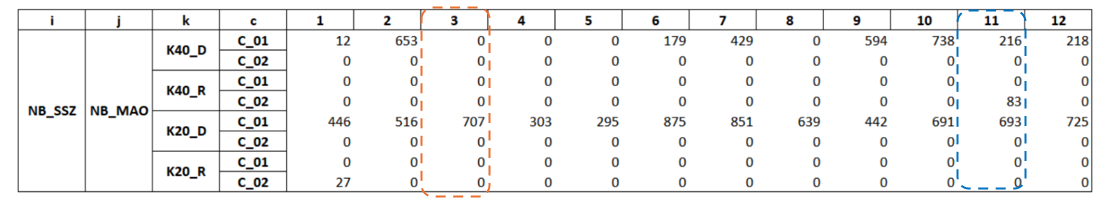
\includegraphics[width=1\linewidth]{RF_SSZ_MAO_2.png}
    \caption{Carga transportada de SSZ para MAO}
    \label{fig:RF_SSZ_MAO}
\end{figure}


Com o aumento do frete para todos os tipos de contêineres, os resultados foram:

\begin{figure}[H]
    \centering
    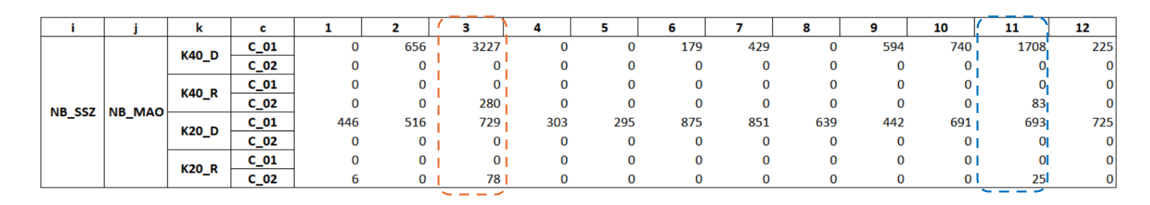
\includegraphics[width=1\linewidth]{RF_SSZ_MAO_3.png}
    \caption{Carga transportada de SSZ para MAO com aumento do frete}
    \label{fig:RF_SSZ_MAO_2}
\end{figure}


Como esperado, o modelo optou por transportar toda a demanda disponível nos períodos alterados (3 e 11), algo que não acontecia no caso padrão.

Também foi utilizado na validação o transporte de contêineres entre PNG e MAO. É uma rota que tem certa demanda, mas praticamente nada é transportado. Abaixo as imagens do caso padrão e aumentando o frete entre esses portos, respectivamente.

\begin{figure}[H]
    \centering
    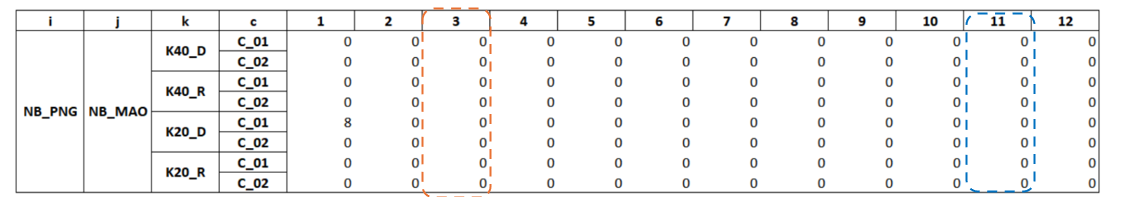
\includegraphics[width=1\linewidth]{RF_PNG_MAO_3.png}
    \caption{Carga transportada de PNG para MAO}
    \label{fig:RF_PNG_MAO}
\end{figure}



\begin{figure}[H]
    \centering
    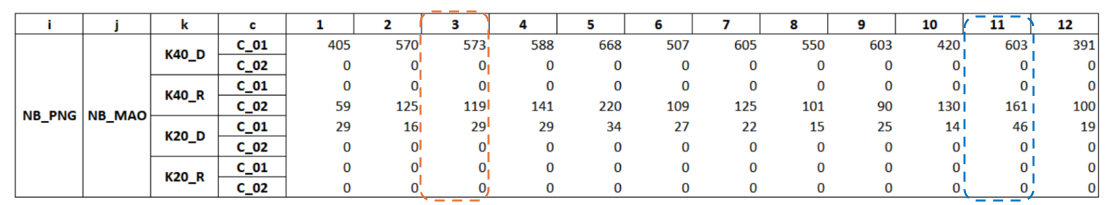
\includegraphics[width=1\linewidth]{RF_PNG_MAO_4.png}
    \caption{Carga transportada de PNG para MAO com aumento do frete}
    \label{fig:RF_PNG_MAO_2}
\end{figure}


Novamente, como esperado, o modelo selecionou toda demanda disponível.

É importante notar que nem sempre um aumento do frete significa que o modelo deve selecionar toda a demanda disponível. Contudo, como o aumento nesta validação foi bem significativo (10 vezes maior) era esperado que toda a demanda fosse selecionada para a movimentação.

\subsection{Variando o Custo}

Outra forma de validar os parâmetros foi reduzir, ou até mesmo considerar como negativo os custos de movimentação de contêineres entre dois portos. Novamente, espera-se que, com os custos reduzidos, a quantidade de contêineres transportados entre determinados portos aumente (e aumente ainda mais caso os custos sejam negativos, o que já que isso representa uma receita financeira para o modelo).

Como exemplo, considerou-se novamente a carga transportada de PNG para MAO. No caso padrão, apenas 8 contêineres foram transportados no primeiro período. Abaixo, a imagem da quantidade transportada após alterar o custo do embarque e desembarque de cheios (CF) entre esses portos para zero.

\begin{figure}[H]
    \centering
    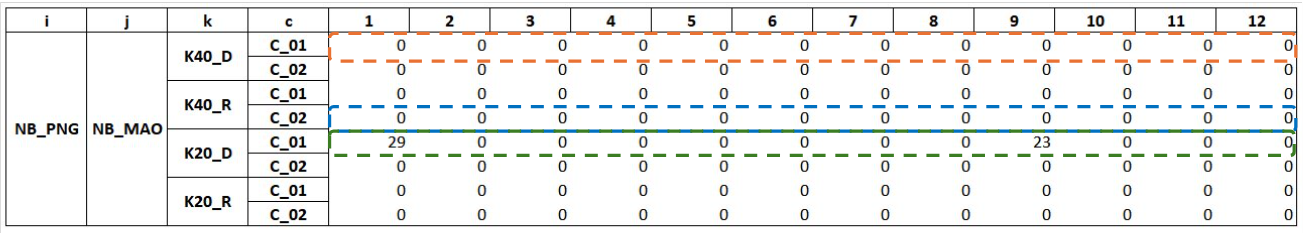
\includegraphics[width=1\linewidth]{figures/CF_0_PNG_MAO.PNG}
    \caption{Carga transportada de PNG para MAO com custo de movimentações zerado}
    \label{fig:CF_0_PNG_MAO}
\end{figure}

A redução de custo não proporcionou um ganho suficiente para que o modelo optasse por levar toda a demanda, mas observa-se que a quantidade de contêineres transportados aumentou, como era esperado. Utilizando um custo negativo, espera-se que a quantidade transportada aumente ainda mais, dado que isso seria o mesmo que aumentar o frete. Abaixo o resultado (com custo multiplicado por uma fator de -3):

\begin{figure}[H]
    \centering
    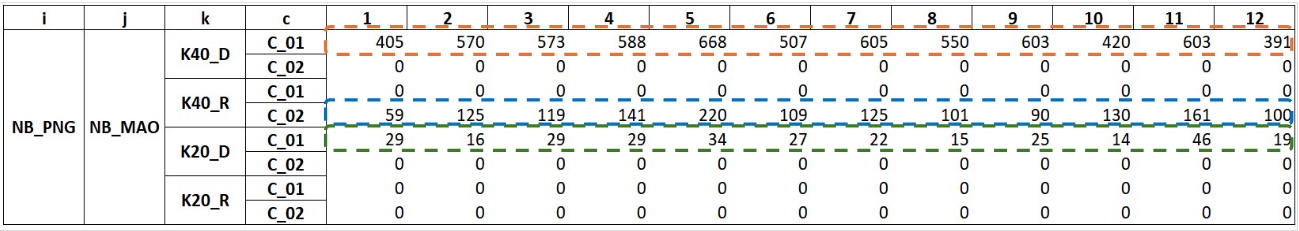
\includegraphics[width=1\linewidth]{figures/CF_NEG_PNG_MAO.PNG}
    \caption{Carga transportada de PNG para MAO com custo de movimentações negativo}
    \label{fig:CF_NEG_PNG_MAO}
\end{figure}

Novamente, uma demanda maior foi selecionada, como era de se esperar. Desta vez, 100\% da demanda.



Ainda alterando o custo de movimentação, mas desta vez ao aumentá-lo, espera-se que a quantidade de contêineres transportados diminua. Para isso, considerou-se o transporte entre PEC e SSZ.

\begin{figure}[H]
    \centering
    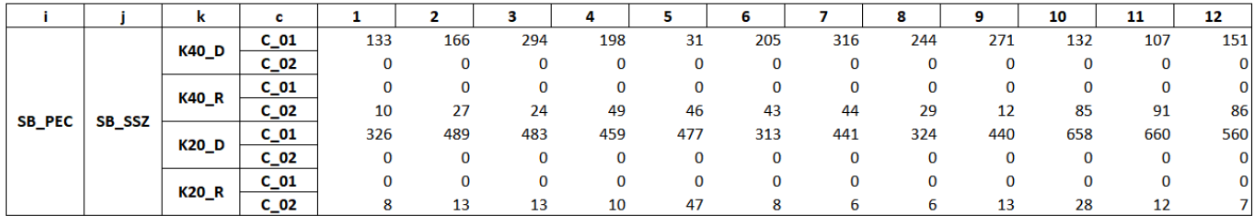
\includegraphics[width=1\linewidth]{figures/CF_PEC_SSZ.PNG}
    \caption{Carga transportada de PEC para SSZ}
    \label{fig:CF_PEC_SSZ}
\end{figure}

Após triplicar os custos relacionados a esse portos, o resultado foi:

\begin{figure}[H]
    \centering
    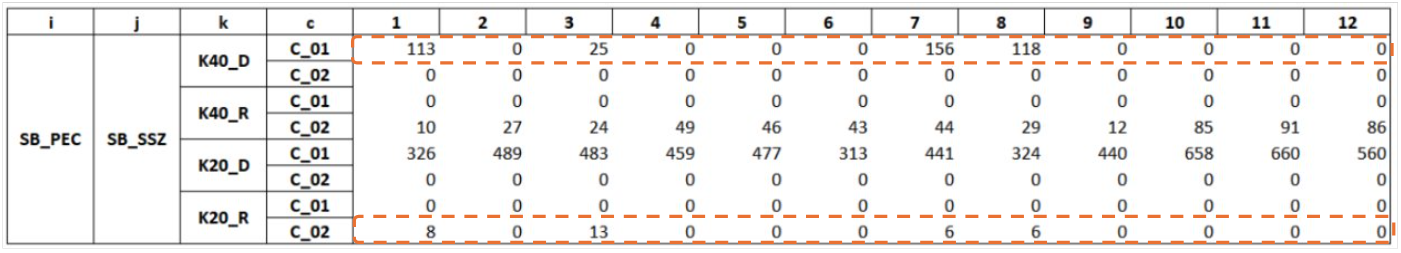
\includegraphics[width=1\linewidth]{figures/CF_PEC_SSZ_2.PNG}
    \caption{Carga transportada de PEC para SSZ com aumento do custo de movimentação}
    \label{fig:CF_PEC_SSZ_2}
\end{figure}

As cargas de contêiner do tipo K20\_D e K40\_R não foram alteradas, mas é possível perceber que os outros tipos de contêineres tiveram o total transportado reduzido.

Pelo limite de refrigerados, os contêineres do tipo K40\_R, que tem maior frete que os K20\_R, são priorizados. Ainda, os de tipo K20\_D também são escolhidos no lugar dos K40\_D, pois há limite de contêineres de 40 pés no navio. Assim, esse espaço foi guardado para transportar contêineres de 40 pés entre portos que não tiveram os custos alterados, e portanto possuem maior margem por unidade transportada.

Finalizando a validação com os custos, considerou-se um cenário em que os custos entre PEC e SSZ utilizados são maiores que o frete entre os portos. Como esperado, nenhum contêiner foi transportado.

\begin{figure}[H]
    \centering
    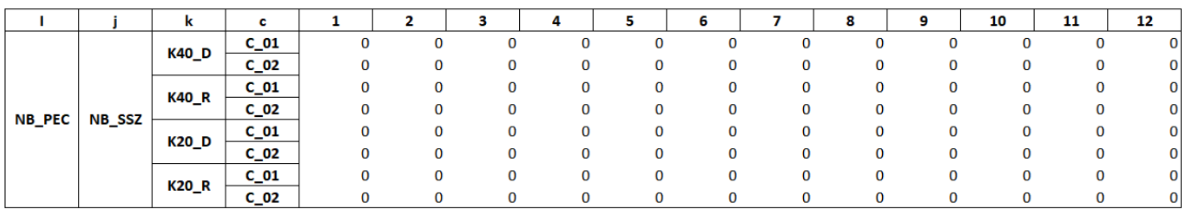
\includegraphics[width=1\linewidth]{figures/CF_PEC_SSZ_3.PNG}
    \caption{Carga transportada de PEC para SSZ com custo de movimentação maior que o frete}
    \label{fig:CF_PEC_SSZ_3}
\end{figure}

\subsection{Contêineres Vazios}

Também deseja-se comparar os resultados obtidos ao aumentar o custo de transporte de contêineres vazios. É esperado que o imbalance dos portos seja corrigido entre portos que não tiveram o custo alterado. A quantidade de contêineres vazios transportados entre os portos no caso base é dada abaixo.

\begin{figure}[H]
    \centering
    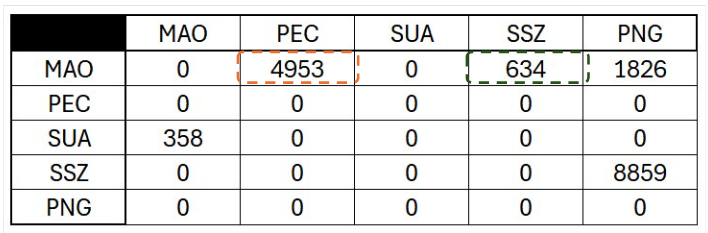
\includegraphics[width=1\linewidth]{figures/CE_geral.PNG}
    \caption{Contêineres vazios reposicionados entre os portos}
    \label{fig:CE_geral}
\end{figure}

Os custos de reposicionamentos dos contêineres de MAO para PEC foram aumentados em três vezes, alterando a matriz de reposicionamento para:

\begin{figure}[H]
    \centering
    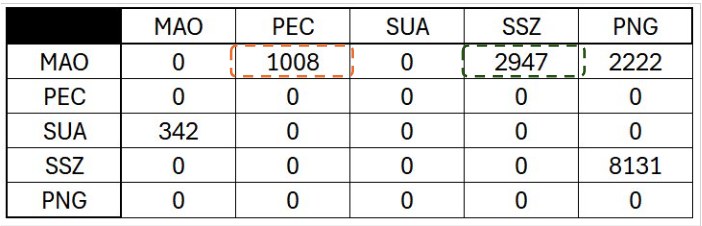
\includegraphics[width=1\linewidth]{figures/CE_geral_0.png}
    \caption{Contêineres vazios reposicionados entre os portos com aumento de custos}
    \label{fig:CE_geral_0}
\end{figure}

Observa-se que o total de contêineres vazios reposicionados para PEC reduziram, enquanto os reposicionados para SSZ aumentaram. Desta forma, é esperado que o total de contêineres cheios exportados de PEC também diminua (de forma a reduzir a necessidade de vazios reposicionados). De fato, esse total foi de ~23950 para ~20610 após o aumento de custos. Por outro lado, com o aumento de transporte desses contêineres para SSZ, a exportação deste porto aumentou, de ~40860 para ~42750, como era de se esperar.

\section{Análise dos resultados}


\subsection{Resultado financeiro}
A proposta na seção de resultados é, considerando um aumento de participação no mercardo progressivo ao longo de 5 anos, definir qual o tipo de navio mais apropriado para a operação nesse ano.

Para isso, em cada um dos 5 anos analisados, o parâmetro Px considerado foi: 15\%, 30\%, 45\%, 60\% e 75\%, sendo que, com os 75\% de participação na rota proposta, obtém-se um market share de aproximadamente 25\%, considerando o mercado de cabotagem como um todo.


Para decidir qual navio será utilizado a partir do ano 5, com a participação de mercado já desenvolvida, foram comparados os resultados e margens operacionais para quatro possíveis navios: 2000, 2500, 3000 e 3500 TEUs.

\begin{figure}[H]
    \centering
    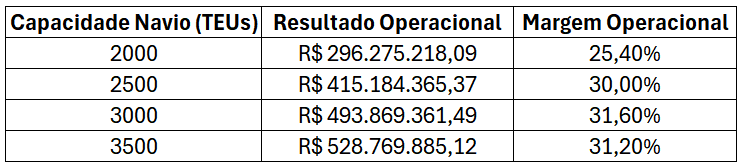
\includegraphics[width=1\linewidth]{figures/ano5_decisao.PNG}
    \caption{Resultados econômicos no 5° ano de operação}
    \label{fig:resultado_navios_ano_5}
\end{figure}

Também optou-se por utilizar um navio menor nos primeiros anos de operação, dada a menor participação de mercado, considerou-se um navio de 2000 TEUs, visando minimizar os prejuízos nos primeiros anos de operação (por conta da baixa participação no mercado). 

Com isso, o próximo passo foi definir em qual ano de operação haveria a mudança do navio menor para o maior. Para isso, utilizou-se a tabela abaixo, que compara os resultados de ambos os navios, ano a ano.

\begin{figure}[H]
    \centering
    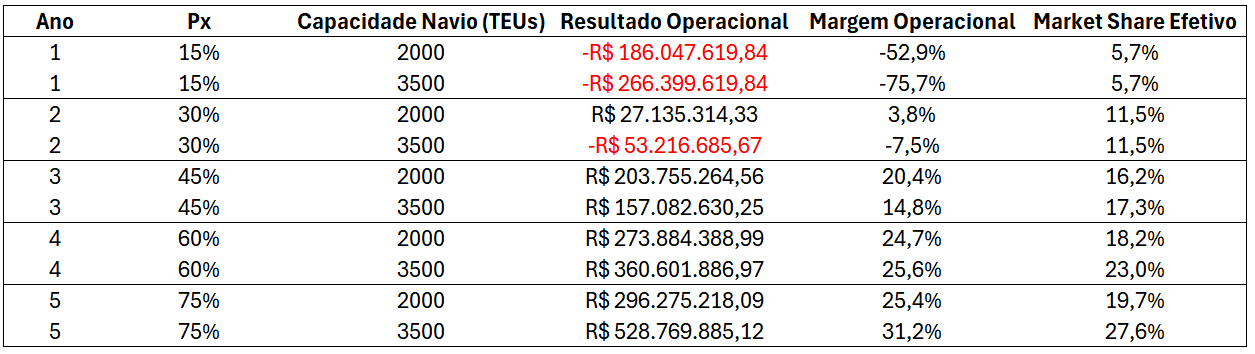
\includegraphics[width=1\linewidth]{figures/opcoes_anos_1_a_5.PNG}
    \caption{Comparação de resultados entre 2000 e 3500 TEUs}
    \label{fig:comparacao_2000_vs_3500}
\end{figure}

Com esses resultados, a decisão foi alterar a frota de navios em operação no quarto ano. Desta forma, o resultado ao longo dos cinco anos foi:

\begin{figure}[H]
    \centering
    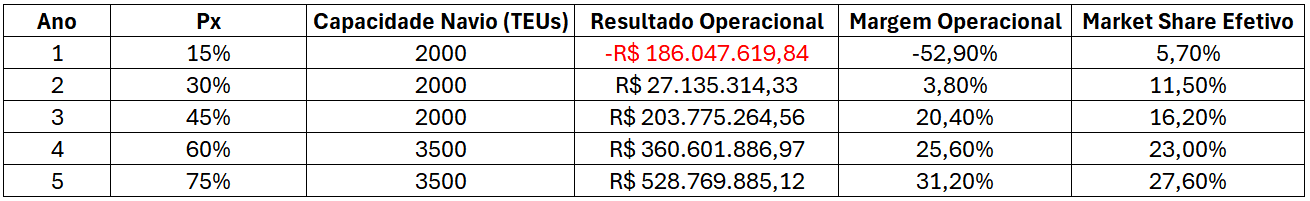
\includegraphics[width=1\linewidth]{figures/ano1_a_5_Decisao.PNG}
    \caption{Resultado Financeiro}
    \label{fig:resultado_financeiro}
\end{figure}

O acumulado da receita e dos custos ao longo dos anos são apresentados abaixo. Com os resultados obtidos, espera-se que a operação atingo o breakeven em 36 meses, durante o terceiro ano de operação, considerando uma custo de capital real de 10\% ao ano.

\begin{figure}[H]
    \centering
    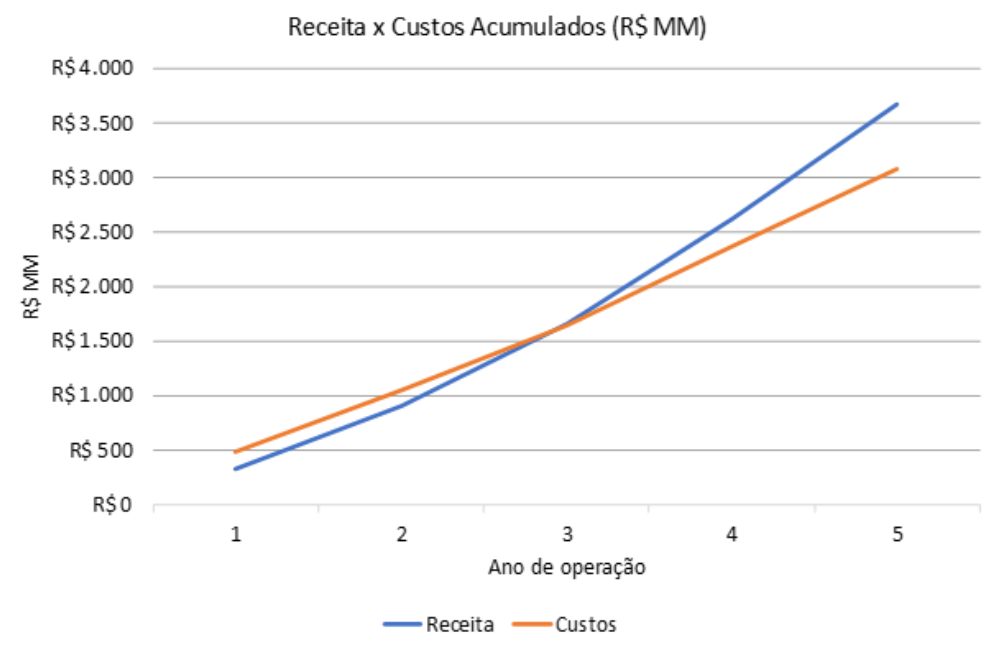
\includegraphics[width=1\linewidth]{figures/receita_vs_custos.png}
    \caption{Evolução da Receita e Custos da Operação}
    \label{fig:receita_vs_custos}
\end{figure}


\subsection{Proforma}

O proforma do modelo, envolvendo as informações de portos de saida e de chegada, assim como as respectivas ocupações do navio, velocidades de navegação, distâncias entre portos, quantidade de embarques e desembarques de contêineres cheios e vazios, tempo de operação e de viagem, receita e custos foi desenvolvido de forma automática pelo grupo. 

O output corresponde à um ciclo de operação, ou seja,  a um mês, sendo que o proforma pode ser gerado para qualquer mês escolhido. É importante ressaltar, também, que os valores são referentes a apenas um navio, porém,  utilizamos 4 navios de igual capacidade para atender o serviço proposto, visando fornecer um serviço semanal.

A seguir, segue o exemplo do proforma de um ciclo de operação no quinto ano para um navio com capacidade de 3500 TEUS:

\begin{figure}[H]
    \centering
    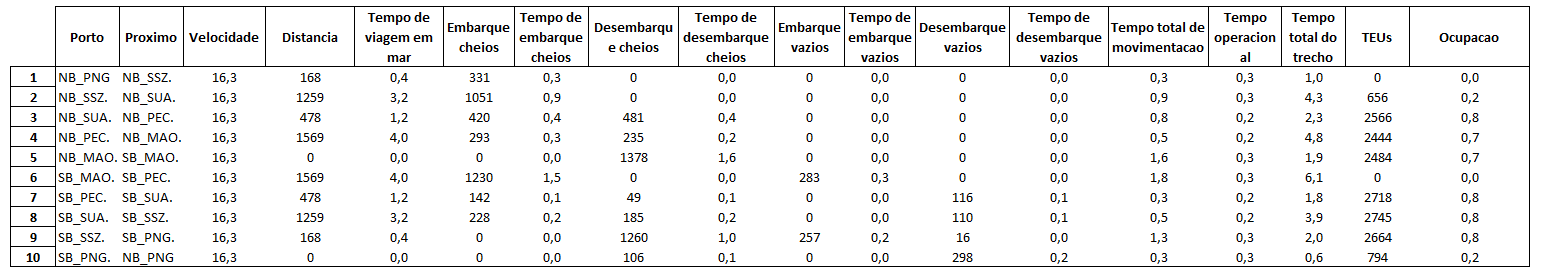
\includegraphics[width=1\linewidth]{proforma1.png}
    \caption{Proforma - Tempos e volume transportado}
    \label{Proforma - Tempos e volume transportado}
\end{figure}


\begin{figure}[H]
    \centering
    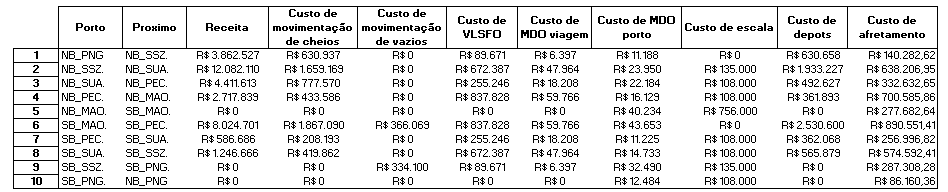
\includegraphics[width=1\linewidth]{proforma2.png}
    \caption{Proforma Receitas e Custos}
    \label{Proforma Receitas e Custos}
\end{figure}

Através dele foi possível calcular também o Slot Cost, referente ao custo de alocação de um contêiner no navio considerado (3500 TEUs), que correspondente à R\$7.324 





\subsection{Custos e Sensibilidade}

 Para decidir qual o custo a ser analisado, foi realizado um cálculo sobre a representatividade de cada tipo de custo no 5° ano de operação, quando a participação do armador está em 75\% e a capacidade do navio é de 3500 TEUs. 


\begin{figure}[H]
    \centering
    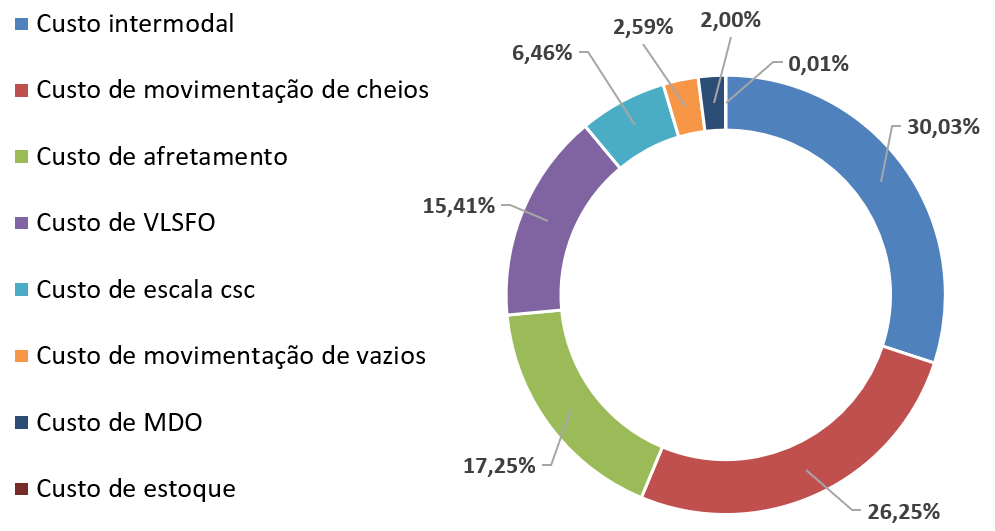
\includegraphics[width=1\linewidth]{figures/sharecustos.png}
    \caption{Share de custos com um navio de 3500 TEUS e 75\% de participação}
    \label{fig:Share custos}
\end{figure}


Foi possível observar que os custos mais representativos são os custos intermodais (30,03\%), referente ao transporte de constêineres entre as capitais dos estados, o custo de movimentação de contêineres cheios e vazios (26,25\%) e o custo de afretamento de navios (17,25\%). Ainda, dólar tem impacto nos custos de combustível (VLSFO e MDO) e afretamento, representando 34,66\% do total.

Dessa forma, devido à grande representatividade, para a análise de sensibilidade decidiu-se variar inicialmente o custo intermodal, que é impactado pela variação de preço do diesel. Aumentando esse custo em 15\%, observou-se uma redução de 9,9\% no resultado operacional, levando a margem para 28,1\% (imagem \ref{fig:aumento_15_intermodal}).

\begin{figure}
    \centering
    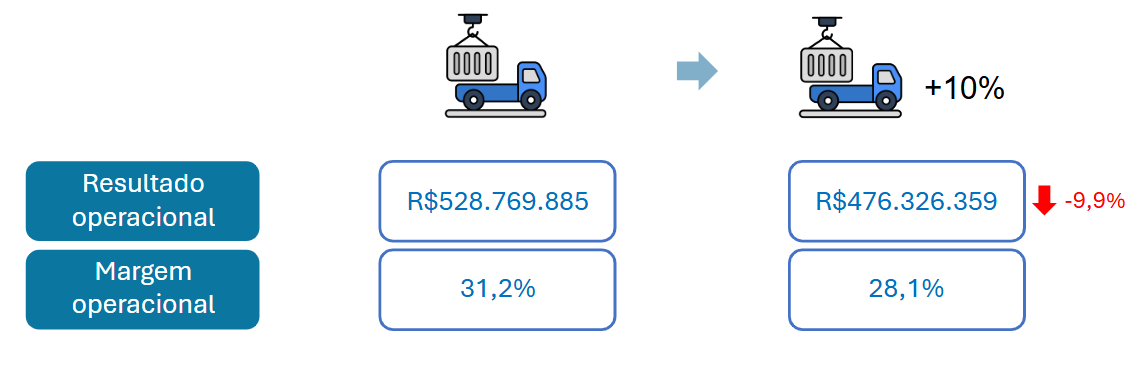
\includegraphics[width=1\linewidth]{figures/aumento_15_intermodal.png}
    \caption{Resultado com aumento de 15\% no custo intermodal}
    \label{fig:aumento_15_intermodal}
\end{figure}

Outro parâmetro escolhido para a análise de sensibilidade foi o preço dos combustível VLSFO e MDO, que são impactados pela variação do preço do barril de petróleo. Considerando um aumento de 15\% no custo dos combustíveis, tem-se um impacto negativo de 5,8\% no resultado operacional (com margem em 29,4\%).

\begin{figure}[H]
    \centering
    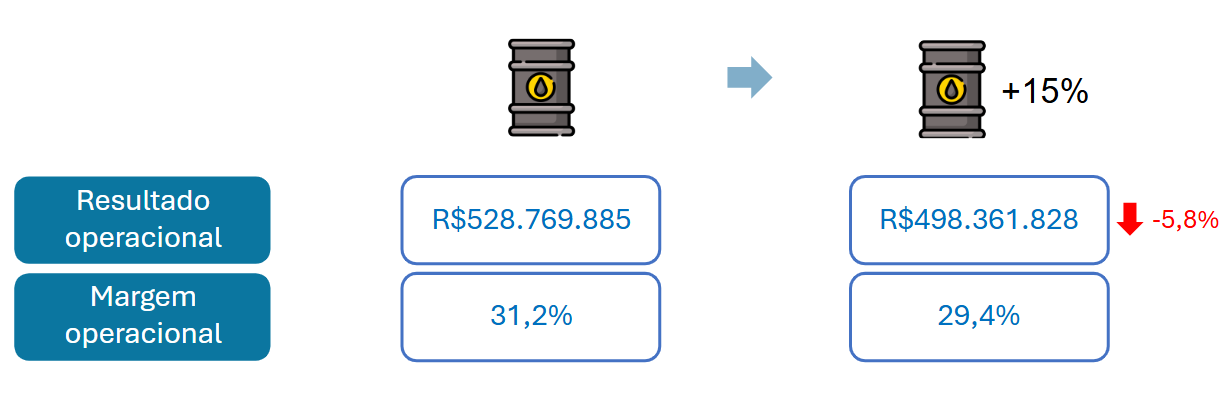
\includegraphics[width=1\linewidth]{figures/aumento_15_combustivel.png}
    \caption{Resultado com aumento de 15\% no preço dos combustíveis}
    \label{fig:aumento_15_combustivel}
\end{figure}


Por fim, devido à volatilidade apresentada nos últimos anos (mostrado na figura \ref{Cotação Dólar}) \cite{dados_abertos_bcb}, junto com a alta representatividade no resultado do modelo, decidiu-se estudar o resultado com a variação do dólar.

\begin{figure}[H]
    \centering
    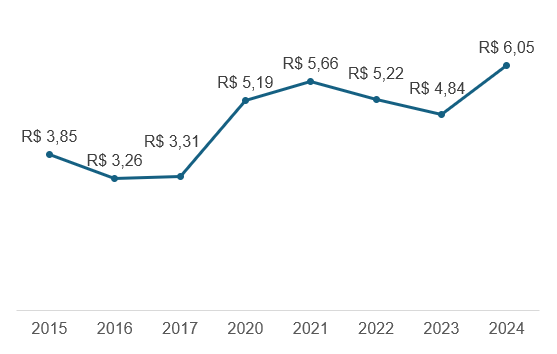
\includegraphics[width=1\linewidth]{figures/cotacao dolar.png}
    \caption{Cotação do dólar ao final de cada ano (valor de 2024 referente ao final do mês de novembro)}
    \label{Cotação Dólar}
\end{figure}

Para tal análise, foi considerado a cotação do Dólar como R\$6,21, um aumento de 15\% em relação ao valor do cenário padrão (R\$ 5,40). Dessa forma, obteve-se uma margem operacional de 27,7\% , o que representa uma redução de 11,5\% no resultado operacional.

\begin{figure}[H]
    \centering
    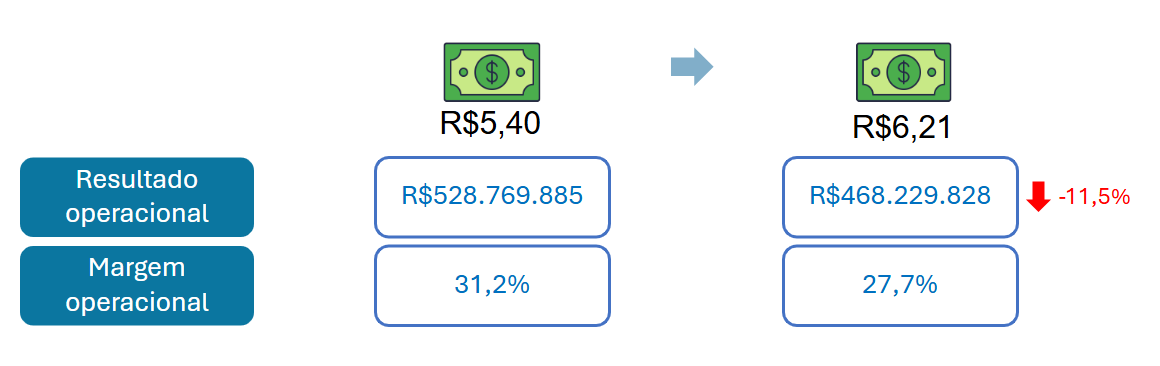
\includegraphics[width=1\linewidth]{figures/aumento_15_dolar.png}
    \caption{Resultado com aumento de 15\% na cotação do dólar}
    \label{fig:aumento_15_dolar}
\end{figure}


\section{Acesso ao código}
O código pode ser acessado no link a seguir: \\ \hyperlink{https://github.com/enzokgomes/PlanejamentoEstocasticoDeRotas}{https://github.com/enzokgomes/PlanejamentoEstocasticoDeRotas}.

%% References with bibTeX database:
% \bibliographystyle{elsarticle-num}
\bibliographystyle{elsarticle-harvard}


\bibliography{references}

\end{document}

